% ch2p8_002: Adding a touch of style
% to grid
% Also exploring parameterization, optional arguments
\documentclass[tikz, border=10pt]{standalone}

\usepackage{tikz}

\tikzset{help lines/.style=very thin}
\tikzset{Karl's grid/.style={help lines, color=blue!50}}

\begin{document}
	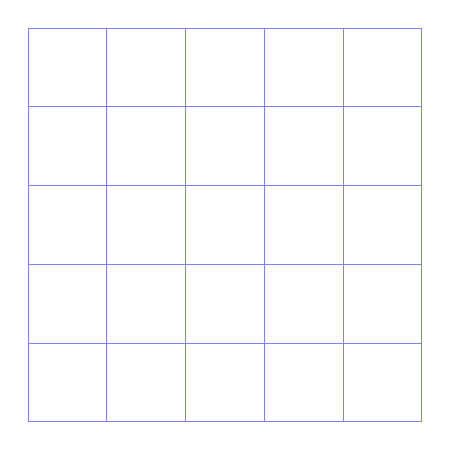
\begin{tikzpicture}
		\draw[Karl's grid] (0, 0) grid (5, 5);
	\end{tikzpicture}
	
	\begin{tikzpicture}[
		Karl's grid/.style={help lines, color=#1!50},
		Karl's grid/.default=blue
		]    % #1 represents first argument for Karl's grid
		% If no argument is passed, default is to used.
		\draw[Karl's grid] (0, 0) grid (1.5, 2);
		\draw[Karl's grid=red] (2, 0) grid (3.5, 2);
	\end{tikzpicture}
\end{document}